\section{图的结构}
\label{sec:graph-structures}

有了顶点集和边集，下一步要问这些局部连接组合出了怎样的整体结构。本节从五个小节依次展开：第~\ref{sec:graph-adjacency-paths}小节把一步的邻接延长为多步的行走、路径、有向无环图与可达关系；第~\ref{sec:graph-euler-hamilton}小节考察不重复边与不重复顶点的全局巡游，即欧拉回路与哈密顿圈；第~\ref{sec:graph-connectivity-separation}小节用可达关系划分连通分量，考察删除顶点或边如何切断连接；第~\ref{sec:graph-cliques-independent-sets}小节考察顶点子集内部“两两相邻”与“两两不相邻”的极端结构，建立团与独立集在补图下的对偶；第~\ref{sec:graph-vertex-cover-dominating}小节讨论如何选出顶点子集监控全部边或支配全部顶点，建立点覆盖与支配集同独立集的关系。

\subsection{邻接与路径}
\label{sec:graph-adjacency-paths}

贯穿图\eqref{eq:graph-conn-running-graph}中顶点$1$和$4$之间没有边，却可以先到$2$或$3$，再到$4$。一步能到谁，由边集直接读出；若干步能到谁，要把边首尾相接。本小节从一个顶点的直接邻居出发，把一步的连接延长为行走和路径，由此得到环、有向无环图以及可达关系。比较不同路线的总长度是第~\ref{chap:shortest-paths}章的问题，这里只讨论哪些顶点序列允许通行。

\subsubsection{邻接、邻域与度}
\label{sec:graph-conn-neighborhoods}

站在一座城市，首先要知道哪些城市与它有直达道路，这样的城市有几座。在无向图中，若$\{i,j\}\in E$，称$i$与$j$\term{邻接}（adjacent），互为邻居。顶点$i$的全部邻居组成它的\term{邻域}（neighborhood）
\[
N(i)=\{j\in V:\{i,j\}\in E\},
\]
邻居的个数$d_i=|N(i)|$称为$i$的\term{度}（degree）。

贯穿图中$N(1)=\{2,3\}$，$N(2)=\{1,3,4\}$，四个顶点的度依次为$2,3,3,2$。度只数直接邻居，经两步才能到达的$4$不计入$N(1)$。

在有向的依赖关系中，还要分清“我直接依赖谁”和“谁直接依赖我”：弧$i\to j$对两端的意义不同。因此分别定义出邻域与入邻域
\[
N^+(i)=\{j:(i,j)\in E\},\qquad
N^-(i)=\{j:(j,i)\in E\},
\]
二者的大小$d_i^+$与$d_i^-$分别称为\term{出度}（out-degree）与\term{入度}（in-degree）。图~\ref{fig:graph-conn-neighborhood-degree}在贯穿图和一个小有向图上标出了这些量。

\begin{figure}[!htb]
  \centering
  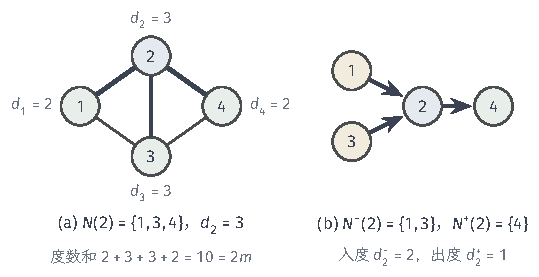
\includegraphics[width=87.669mm]{figures/01-basic-mathematics/04-graphs/tikz/c1-neighborhood-degree/figure.pdf}
  \caption{邻域与度。(a)贯穿图中顶点$2$的邻域$N(2)=\{1,3,4\}$（绿色），连接它们的三条边加粗，所以$d_2=3$；顶点旁标出各点的度，四个度之和$10$恰为边数的两倍。(b)有向图$1\to2$、$3\to2$、$2\to4$中，顶点$2$的入邻域$N^-(2)=\{1,3\}$（黄色）与出邻域$N^+(2)=\{4\}$（绿色），入度为$2$，出度为$1$。}
  \label{fig:graph-conn-neighborhood-degree}
\end{figure}

\paragraph{度数和与边数}
考虑所有“顶点—边”配对$(i,e)$，其中$i$是边$e$的端点。按顶点分组，顶点$i$出现在$d_i$个配对中；按边分组，每条边恰有两个端点。两种分组数的是同一批配对，所以
\begin{equation}
\sum_{i\in V}d_i=2m.
\label{eq:graph-conn-handshake}
\end{equation}
由此可知度为奇数的顶点个数必是偶数。有向图中每条弧恰好贡献一个出度和一个入度，所以$\sum_i d_i^+=\sum_i d_i^-=m$。

\paragraph{邻域与度的读取}
给每个顶点准备一个空的邻居集合和一个初始为$0$的计数器，然后逐条读边：读到$\{i,j\}$时，把$j$放进$N(i)$、$i$放进$N(j)$，两个计数器各加$1$。表~\ref{tab:graph-conn-degree-trace}是贯穿图上计数器的变化。每读一条边，度数和加$2$，读完$m$条边就是$2m$，这正是式\eqref{eq:graph-conn-handshake}；最后一列若不等于两倍已读边数，说明计数存在遗漏或重复；只记一端是可能的原因之一。

有向图读到弧$(i,j)$时，把$j$放进$N^+(i)$、$i$放进$N^-(j)$。图~\ref{fig:graph-conn-direction-orientation}(c)的$1\to2\leftarrow3$读完后$N^-(2)=\{1,3\}$，$N^+(2)=\varnothing$；不说明方向，就可能把入邻居误当成下一步可以到达的顶点。这里的度只数结构上的边；边带权时把一个顶点所有邻边的权相加，得到的是另一个量，本部分不使用。

\begin{table}[!htb]
  \centering
  \small
  \begin{tabular}{@{}lccccc@{}}
    \toprule
    已读入的边 & $d_1$ & $d_2$ & $d_3$ & $d_4$ & 度数和\\
    \midrule
    初始 & $0$ & $0$ & $0$ & $0$ & $0$\\
    $\{1,2\}$ & $1$ & $1$ & $0$ & $0$ & $2$\\
    $\{1,3\}$ & $2$ & $1$ & $1$ & $0$ & $4$\\
    $\{2,3\}$ & $2$ & $2$ & $2$ & $0$ & $6$\\
    $\{2,4\}$ & $2$ & $3$ & $2$ & $1$ & $8$\\
    $\{3,4\}$ & $2$ & $3$ & $3$ & $2$ & $10$\\
    \bottomrule
  \end{tabular}
  \caption{逐条读入贯穿图的边时，四个度计数器的变化。每读一条边，恰有两个计数器各加$1$，度数和每次增加$2$。}
  \label{tab:graph-conn-degree-trace}
\end{table}

\subsubsection{行走、路径与环}
\label{sec:graph-conn-walks-paths}

走一步就是从当前顶点走到它的一个邻居，走若干步就得到一串相邻两项都邻接的顶点。是否允许重复经过顶点要看用途：计数多步走法时允许重复，一条实际路线通常不允许。

\begin{definition}[行走与路径]
\label{def:graph-conn-walk-path}
设$\mathcal G=(V,E)$是无向图。顶点序列$(v_0,\ldots,v_k)$若对每个$r=1,\ldots,k$都有$\{v_{r-1},v_r\}\in E$，就称为从$v_0$到$v_k$的一条\term{行走}（walk），$k$称为它的长度，即经过的边数。若行走中的顶点两两不同，就称为一条简单\term{路径}（path）。
\end{definition}

单个顶点$(v_0)$是长度为零的行走，也是长度为零的路径。本部分不加修饰的“路径”都指简单路径。

绕一圈回到起点的路线还要与原路折返区分开。首尾相同（$v_0=v_k$）的行走称为\term{闭行走}（closed walk），但闭合不意味着绕成一圈：沿一条边去而复返的$(2,4,2)$是闭行走，却没有提供第二条路线。

因此把长度$k\geq3$、且$v_0,\ldots,v_{k-1}$两两不同的闭行走称为\term{环}（cycle）；长度为$1$的闭行走需要自环，长度为$2$的只能沿同一条边往返，所以要求$k\geq3$。同一个环可以从不同顶点出发、沿两个方向书写，例如$(1,2,3,1)$与$(1,3,2,1)$，我们把经过同一组边的序列看成同一个环。

\paragraph{顶点序列的核对}
判断一个顶点序列属于哪一类，按定义依次检查：每一步$\{v_{r-1},v_r\}$是否为边，判断行走；从左到右维护“已出现顶点”的集合，看有无重复，判断路径；再要求$k\geq3$、首尾相同且前$k$个顶点不重复，判断环。

图~\ref{fig:graph-conn-walk-path-cycle}给出四个结果：$(1,2,3,1,2)$是行走，但第二次读到$1$时重复，不是路径；$(1,2,4)$是路径；$(2,4,2)$是闭行走而不是环；$(1,2,3,1)$是环。

路径和环都是特殊的行走，但二者的限制不同：路径不重复任何顶点，环则要求首尾相同、其余顶点互异。行走便于拼接与计数，路径给出不重复顶点的路线，环提供替代路线。

\begin{figure*}[!htb]
  \centering
  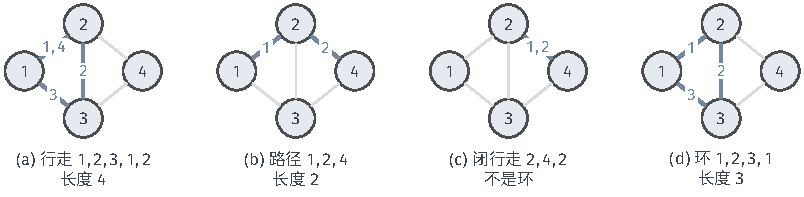
\includegraphics[width=136.186mm]{figures/01-basic-mathematics/04-graphs/tikz/c1-walk-path-cycle/figure.pdf}
  \caption{贯穿图上的四种顶点序列。蓝色粗线是经过的边，边旁数字是经过该边的步序，浅灰色是未经过的边。(a)行走可以重复经过边$\{1,2\}$；(b)路径不重复顶点；(c)沿一条边去而复返得到闭行走，但它不是环；(d)绕三角形一周的环除首尾外不重复顶点。}
  \label{fig:graph-conn-walk-path-cycle}
\end{figure*}

\subsubsection{有向路径与有向无环图}
\label{sec:graph-conn-dag}

任务依赖要求每一步都顺着箭头走。若顺着箭头走一圈又回到出发的任务，例如$1$等$2$、$2$等$3$、$3$又等$1$，这组任务就无法按任何次序全部完成。把定义~\ref{def:graph-conn-walk-path}中的条件换成$(v_{r-1},v_r)\in E$，就得到有向行走与\term{有向路径}（directed path）。除首尾外顶点两两不同、长度至少为$1$的有向闭行走称为\term{有向环}（directed cycle）；由于没有自环，其长度至少为$2$。

\begin{definition}[有向无环图]
\label{def:graph-conn-dag}
不含有向环的有向图称为\term{有向无环图}（directed acyclic graph，DAG）。
\end{definition}

有向环的最短长度与无向情形不同。图~\ref{fig:graph-conn-directed-cycle-dag}(a)中两条反向弧$i\to j$和$j\to i$是两个不同的对象，$(i,j,i)$构成长度为$2$的有向环；无向图中的$(2,4,2)$两次经过的是同一条边。图(b)的$(1,2,3,1)$每一步都顺着箭头，是长度为$3$的有向环。

\begin{figure}[!htb]
  \centering
  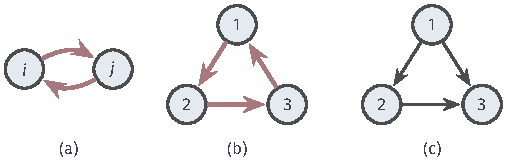
\includegraphics[width=85.687mm]{figures/01-basic-mathematics/04-graphs/tikz/c1-directed-cycle-dag/figure.pdf}
  \caption{有向环与有向无环图。红色弧组成有向环。(a)两条反向弧构成长度为$2$的有向环；(b)三角形的循环定向含有向环；(c)同一个三角形的另一种定向不含有向环，是有向无环图，尽管它的底层无向图是一个环。}
  \label{fig:graph-conn-directed-cycle-dag}
\end{figure}

\paragraph{无环的核对}
有向环上的每个顶点都有环上的弧进出，所以入度或出度为$0$的顶点不在任何有向环上。图~\ref{fig:graph-conn-directed-cycle-dag}(c)的弧为$1\to2$、$1\to3$、$2\to3$，$1$的入度与$3$的出度为$0$，剩下的顶点$2$不足以构成至少含两个顶点的有向环，所以它是DAG。大图上系统地判断有无有向环，要用第~\ref{sec:graph-dfs}节的深度优先遍历或第~\ref{sec:graph-topological-order}节的拓扑排序。

图(c)是DAG，它的底层无向图却是三角形。拓扑排序要求的正是有向无环；若改用“底层无向图无环”判定，就会错误地排除(c)。反过来，允许一对反向弧时，底层无向图即使是一条边，也可能含有长度为$2$的有向环。因此，这两个无环条件一般并不等价。

\subsubsection{可达性}
\label{sec:graph-conn-reachability}

很多问题只关心从$i$出发能不能到达$j$，而不关心怎么到。若存在从$i$到$j$的行走，称$j$从$i$\term{可达}（reachable）；有向图中要求有向行走。行走首尾相接仍是行走，路径则未必，所以用行走定义更方便。下面的引理说明改用路径定义并无区别。

\begin{lemma}[行走中含有路径]
\label{lem:graph-conn-walk-contains-path}
在无向图或有向图中，若存在从$i$到$j$的行走，则存在从$i$到$j$的路径，并且它的顶点和边都取自这条行走。
\end{lemma}

\begin{proof}
在从$i$到$j$、顶点和边都取自原行走的所有行走中，取长度最短的一条$(v_0,\ldots,v_k)$。若它不是路径，则有$s<t$使$v_s=v_t$。删去中间段$v_{s+1},\ldots,v_t$，得到$(v_0,\ldots,v_s,v_{t+1},\ldots,v_k)$：原来从$v_t$出发的那一步现在从$v_s=v_t$出发，每一步仍沿原有的边或弧，而长度减少了$t-s>0$，矛盾。
\end{proof}

\paragraph{从行走中取出路径}
实际取出路径时，可以从左到右读一遍行走，随读随删。维护当前路径$P$，初始为$(v_0)$，并给$P$上的顶点做标记。读到$v_r$时，若它没有标记，就接到$P$末尾；若已有标记，说明$P$绕回了$v_r$，就把$P$截到$v_r$所在的位置，并清除其后的标记。$P$始终顶点互异、各边取自原行走，读完时就是所求的路径。同一顶点可能多次加入、删去，但行走中的每次出现至多引起一次加入，而每个加入的记录至多删除一次。用栈保存当前路径并记录各顶点在栈中的位置后，总工作量与行走长度成正比。

以行走$(1,2,3,1,3,4)$为例，$P$依次为$(1)$、$(1,2)$、$(1,2,3)$，读到第二个$1$时截回$(1)$，再变为$(1,3)$、$(1,3,4)$。

图~\ref{fig:graph-walk-erasure}把这一步删除单独展开。两次出现的顶点$1$使中间一段闭合；删去这段绕行后，后续的$1,3,4$仍逐边相接，起点和终点都不变。

\begin{figure}[!htb]
  \centering
  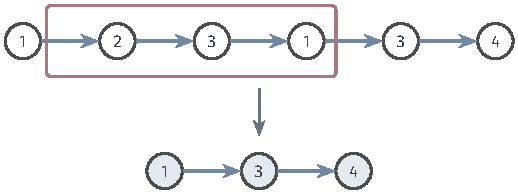
\includegraphics[width=87.669mm]{figures/03-graphs/01-structure-and-computation/tikz/walk-erasure/figure.pdf}
  \caption{从行走中删去重复段。上排按行走次序展开为$(1,2,3,1,3,4)$，同号圆点表示同一个原图顶点；红框圈出被删去的后一次$1$及其前面的绕行部分。下排得到路径$(1,3,4)$。箭头仅表示读取次序，不给原无向图增加方向。}
  \label{fig:graph-walk-erasure}
\end{figure}

\paragraph{可达关系的性质}
零长度行走给出自反性，行走首尾相接给出传递性；无向图中把行走倒过来走仍是行走，所以还有对称性。同时满足自反、对称、传递三条的二元关系称为等价关系，所以无向图上的可达关系是等价关系。等价关系的等价类两两不交、并起来恰为全集，第~\ref{sec:graph-connectivity-separation}小节据此划分连通分量；等价关系与划分的一般对应，可参考\BookChapterRef{chap:sets-relations-maps}{卷一第~\ref{chap:sets-relations-maps}章}。

这里的性质只说明可达关系是什么。给出两个具体顶点、要判断是否可达，仍需要有组织地访问能走到的顶点，这是第~\ref{sec:graph-bfs}节与第~\ref{sec:graph-dfs}节的任务。

有向图中倒过来走需要反向弧，对称性不再成立：单向链$1\to2\to3$中，$3$从$1$可达，$1$却不从$3$可达。为描述这种单向关系，$N^-(j)$中的顶点称为$j$的直接\term{前驱}（predecessor），$N^+(j)$中的顶点称为直接\term{后继}（successor）；能经一条或多条弧到达$j$的其他顶点称为$j$的\term{祖先}（ancestor），从$j$出发经一条或多条弧能到达的其他顶点称为$j$的\term{后代}（descendant）。本部分约定祖先与后代都不含$j$自身。

单向链中$3$的直接前驱只有$2$，祖先是$\{1,2\}$；$1$的后代是$\{2,3\}$。

有向环上的两个不同顶点可以互为祖先，在DAG中这不可能发生：若$i\neq j$互为祖先，两条有向路径拼成长度至少为$2$的有向闭行走$(v_0,\ldots,v_k)$；在所有满足$s<t$、$v_s=v_t$的位置对中取$t-s$最小的一对，$(v_s,\ldots,v_t)$除首尾外不重复顶点，长度又不能为$1$，所以是有向环，矛盾。可达的不对称使有向图的“连通”需要两种定义，这将在第~\ref{sec:graph-connectivity-separation}小节讨论。

\subsection{欧拉回路与哈密顿圈}
\label{sec:graph-euler-hamilton}

行走对顶点和边都不禁重复，简单路径和环则禁止重复顶点。在实际巡检与路线规划中，还有两类常见的全局遍历要求：一类是像洒水车清扫全部街道那样，要求把图中的每一条边都恰好走过一次，允许重复经过同一个路口；另一类是像邮递员投递全部站点那样，要求把图中的每一个顶点都恰好访问一次，不需要走遍所有道路。这两类问题在叙述上只把“每条边一次”换成了“每个顶点一次”，背后的图结构与计算难度却截然不同。

\subsubsection{欧拉迹与欧拉回路}
\label{sec:graph-euler-circuit}

先考察不重复边的巡游。清扫道路网时，只要把所有道路都清扫一遍即可，中间可以多次经过同一个路口。

\begin{definition}[欧拉迹与欧拉回路]
\label{def:graph-euler-circuit}
设$\mathcal G=(V,E)$是无向图。若一条行走恰好经过$E$中的每条边各一次，就称为一条\term{欧拉迹}（Eulerian trail）；首尾顶点相同的欧拉迹称为\term{欧拉回路}（Eulerian circuit）。
\end{definition}

一个图何时存在欧拉回路？不妨观察行走经过某个顶点$v$时的局部动作：每次沿着一条边进入$v$，只要还没有停下，就必须沿着另一条尚未走过的边离开$v$；即使$v$是起点兼终点，最开始从$v$出发的一步与最后回到$v$的一步也恰好配成一对。这意味着，欧拉回路每经过顶点$v$一次，就会消耗掉与$v$关联的两条边。要让所有边都被不重不漏地走完，每个顶点的度都必须是偶数。下面的定理表明，对于连通无向图，这个一眼就能看出的局部条件同时也是充分条件。

\begin{theorem}[无向图欧拉回路的判别]
\label{thm:graph-euler-circuit}
设$\mathcal G=(V,E)$是至少有一条边的连通无向图。$\mathcal G$存在欧拉回路，当且仅当每个顶点$v\in V$的度$d_v$都是偶数。
\end{theorem}

\begin{proof}
先证必要性。设$W=(v_0,v_1,\ldots,v_m)$是$\mathcal G$的一条欧拉回路，其中$v_m=v_0$。在$W$中，顶点$v\neq v_0$每出现一次，它的前一步边$\{v_{r-1},v\}$与后一步边$\{v,v_{r+1}\}$就组成一对关联于$v$的不同边；起点$v_0$在中间每出现一次同样配成一对边，再加上首步边$\{v_0,v_1\}$与末步边$\{v_{m-1},v_0\}$又配成一对。因为$E$中每条边在$W$中恰好出现一次，所以关联于每个顶点$v$的边都两两配对，即$d_v$必为偶数。

再证充分性，证明过程给出构造欧拉回路的Hierholzer闭行走拼接思路由来。对边数$m$用归纳法，或直接按如下方式逐步扩张闭行走。任取起点$u_0\in V$，沿尚未走过的边一步步前进，且绝不重复使用已走过的边。每当走到一个顶点$v\neq u_0$时，此前已经离开并进入$v$若干次，再加上刚刚进入$v$的这一步，关联于$v$的已用边数是奇数；而$d_v$是偶数，所以$v$处一定还剩至少一条未用边可供继续前进。由此可见，只要没有回到$u_0$，行走就绝不会在中途被困住；由于总边数$m$有限，它必定在有限步后回到$u_0$，停下时得到一条不重复边的闭行走$C_0$。

若$C_0$已经包含了$E$的全部边，它就是欧拉回路。否则，从$\mathcal G$中删去$C_0$用掉的边，记剩余边组成的子图为$\mathcal G'$。因为$C_0$在每个顶点处用掉的边数都是偶数，所以$\mathcal G'$中每个顶点的度仍然是偶数；又因为原图$\mathcal G$连通，已走过的闭行走$C_0$与剩余边集之间必有公共顶点$w$，它在$\mathcal G'$中仍有未用邻边。以$w$为起点在$\mathcal G'$中按同样规则走出一条不重复边的闭行走$C_1$，再把$C_0$经过$w$的位置拆开、嵌入$C_1$，就拼成了一条更长的不重复边闭行走。每次拼接至少多吸收一条边，至多$m$步就能将全部边拼成一条欧拉回路。
\end{proof}

若允许起点$s$与终点$t$不同（$s\neq t$），则除$s$首次出发的一步和$t$最后到达的一步外，其余每次进出顶点仍两两配对。同理可知，连通无向图存在起终点不同的欧拉迹，当且仅当恰有两个顶点的度为奇数，其余顶点的度均为偶数。在贯穿图\eqref{eq:graph-conn-running-graph}中，四个顶点的度依次为$2,3,3,2$：因为$d_2=d_3=3$是奇数，贯穿图没有欧拉回路；但奇度顶点恰有$2$和$3$两个，所以存在以$2,3$为两端的欧拉迹，例如$(2,1,3,2,4,3)$恰好把五条边各走一次。

\subsubsection{哈密顿路径与哈密顿圈}
\label{sec:graph-hamilton-cycle}

把要求从“每条边恰好一次”改为“每个顶点恰好一次”，就得到哈密顿问题。

\begin{definition}[哈密顿路径与哈密顿圈]
\label{def:graph-hamilton-cycle}
设$\mathcal G=(V,E)$是无向图。包含$V$中全部顶点的简单路径称为\term{哈密顿路径}（Hamiltonian path）；包含$V$中全部顶点的环称为\term{哈密顿圈}（Hamiltonian cycle）。
\end{definition}

贯穿图\eqref{eq:graph-conn-running-graph}有$4$个顶点，环$(1,2,4,3,1)$依次经过全部四个顶点且首尾闭合，因此是一个哈密顿圈，边$\{2,3\}$则被舍弃不用。

什么样的图一定存在哈密顿圈？直观上，图中的边越稠密、每个顶点的邻居越多，就越容易把所有顶点串成一个大环。记$\delta(\mathcal G)=\min_{v\in V}d_v$为图$\mathcal G$的最小度，下面的Dirac定理给出了一个经典的充分条件。

\begin{theorem}[Dirac定理]
\label{thm:graph-dirac-hamilton}
设$\mathcal G=(V,E)$是有$n\geq 3$个顶点的简单无向图。若每个顶点的度都至少为$n/2$，即$\delta(\mathcal G)\geq n/2$，则$\mathcal G$必存在哈密顿圈。
\end{theorem}

\begin{proof}
先说明$\mathcal G$必连通：若有两个连通分量，较小分量的顶点数至多为$n/2$，其中任一顶点的邻居都在该分量内部，度至多为$n/2-1$，与$\delta(\mathcal G)\geq n/2$矛盾。

在$\mathcal G$的所有简单路径中取一条长度最大的路径$P=(v_0,v_1,\ldots,v_k)$。因为$P$不能再向两端延长，起点$v_0$和终点$v_k$的全部邻居都已经在$P$上，即$N(v_0)\subseteq\{v_1,\ldots,v_k\}$且$N(v_k)\subseteq\{v_0,\ldots,v_{k-1}\}$。考虑下标集合
\[
I=\bigl\{r\in\{1,\ldots,k\}:\{v_0,v_r\}\in E\bigr\},\qquad
J=\bigl\{r\in\{1,\ldots,k\}:\{v_{r-1},v_k\}\in E\bigr\}.
\]
因为$|I|=d_{v_0}\geq n/2$且$|J|=d_{v_k}\geq n/2$，而$I,J$都是$\{1,\ldots,k\}$（共$k\leq n-1$个元素）的子集，由抽屉原理，
\[
|I\cap J|=|I|+|J|-|I\cup J|\geq \frac{n}{2}+\frac{n}{2}-(n-1)=1.
\]
于是存在下标$r\in I\cap J$，使得$\{v_0,v_r\}\in E$且$\{v_{r-1},v_k\}\in E$。把路径$P$在$v_{r-1}$与$v_r$之间断开，改用这两条边连接，就得到一个包含$P$中全部$k+1$个顶点的环
\[
C=(v_0,v_1,\ldots,v_{r-1},v_k,v_{k-1},\ldots,v_r,v_0).
\]

若$k+1=n$，则$C$已是哈密顿圈。若$k+1<n$，由$\mathcal G$连通，必有环外顶点$w$与$C$上某个顶点$v_s$相邻；先从$w$沿边走到$v_s$，再沿$C$的一个方向依次访问其余环上顶点，在回到$v_s$之前停下，就得到一条含$k+2$个顶点的简单路径，与$P$最长矛盾。因此必有$k+1=n$，$C$即为哈密顿圈。
\end{proof}

\paragraph{为什么从欧拉回路到哈密顿圈难度骤增}
对比定理~\ref{thm:graph-euler-circuit}与定理~\ref{thm:graph-dirac-hamilton}可以看出两个判定问题的计算差异：判断一张图有没有欧拉回路，只需数出每个顶点的度是否全为偶数并检查连通性，在与顶点数加边数成正比的$O(n+m)$时间内完成判定；而Dirac定理只给出了哈密顿圈的一个充分条件（贯穿图\eqref{eq:graph-conn-running-graph}满足$d_v\geq 2=4/2$，但很多度数很小的图如长为$n$的单环本身也是哈密顿圈），图论中至今没有找到好算的哈密顿圈充要判据，判定一般图是否存在哈密顿圈是著名的NP完全问题。

这一计算复杂度差异的一个结构原因，在于“每条边一次”是局部守恒条件，而“每个顶点一次”是全局取舍条件。在欧拉回路问题中，所有边都必须被用上，不存在“选哪条边、舍弃哪条边”的抉择；只要每个顶点的度都是偶数，无论前面怎么走，只要还没有回到起点，当前顶点剩下的未用邻边就一定还有至少一条，局部走出的任何闭行走都可以通过Hierholzer拼接无损地合入全局回路，永远不会因为“走错一步”而把后面的路堵死。

相反，哈密顿圈要从$m$条边中只挑出$n$条边围成单环，每经过一个顶点$v$，它关联的其余$d_v-2$条边就被迫全部作废。一次看似合法的局部前进，可能在不知不觉中删光了远处某个顶点的可用邻边，或者把尚未访问的顶点切成几个互不相连的碎片，必须退回重选。局部度数完全看不出这种全局瓶颈：例如把两个三角形用一条桥连起来（或取两个三角形共用一个割点），每个顶点的度都至少为$2$，但任何走法一旦跨过桥或经过割点，就再也无法在不重复顶点的前提下回到另一侧。正是这种“局部选择牵动全局连通性”的耦合，使哈密顿圈无法像欧拉回路那样靠局部度数判别。
